Dieser Abschnitt soll eine kleine Demo einzelner Funktionalitäten darstellen, indem die jeweiligen Beispiele in einem Kontext vorgestellt werden.
\footcite[An dieser Stelle soll erneut auf die Lizenz hingewiesen werden. Siehe][]{ccOJlizenz}
Für Grundlegendes kann sowohl die README als auch das Latex-Sheet zu Rate gezogen werden. 
Über die einzelnen Themen sind Verwendungen von Abkürzungen und Fußnoten wie dieser\footrefnote{Lipsum}{lipsum} verteilt. 

Zeilenumbrüche in der PDF können entweder mittels zwei Zeilenumbrüche in der Quelldatei erzeugt werden, wie vor dieser Zeile.\\
Oder durch doppelten Backslash, wie vor dieser Zeile.

\subsection{Fließelemente}
  \begin{wrapfigure}{r}{0.45\linewidth}
    \centering
    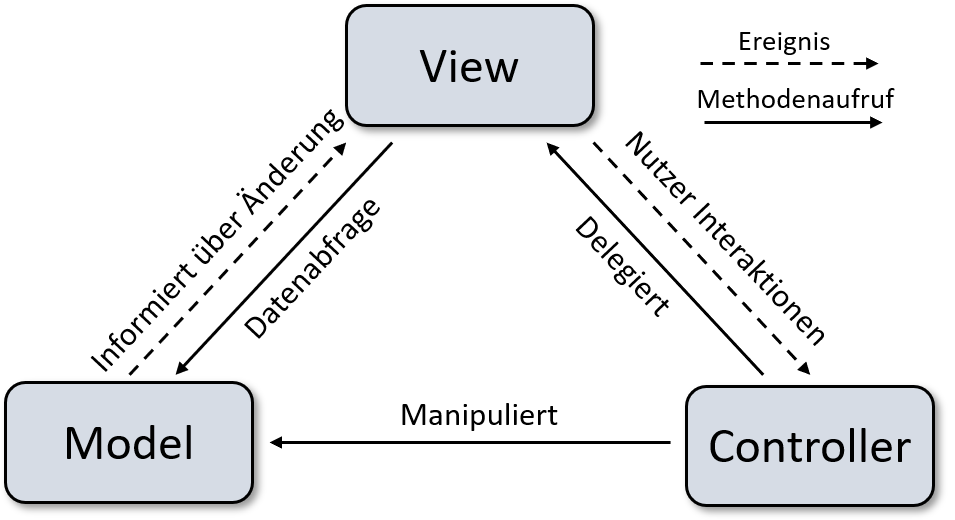
\includegraphics[width=0.45\textwidth]{mvc}
    % caption[im Verzeichnis]{unter der Abbildung}
    \caption[Aufbau von \acrlong{MVC}]{Aufbau von \gls{MVC}.\\Quelle: Angelehnt an \cite{curry2008flexible}}
    \label{fig_mvc}
  \end{wrapfigure}

  Diese umfassen Bilder, Tabellen sowie Listings.
  Während sich das Beispiel für Listings im Anhang~\ref{appendix_dummy} befindet, zeigt dieses Kapitel die Nutzung der anderen Elemente auf.

 \subsubsection{Bilder}
    Bilder können sowohl als eigenständiges Blockelement, als auch mit dem Text in einer Zeile mit fließen.
    Jedoch entscheidet \LaTeX wo genau die Bilder angezeigt werden, weshalb sie nicht unbedingt an der Stelle erscheinen,
    an der sie definiert wurden.
    Jedoch können (und sollten) im Text über das vergebene Label referenziert werden:

    Durch diese Verbindungen entsteht eine Dreiecksform, welche in Abbildung~\ref{fig_mvc} illustriert wird.

    \begin{figure}[tbh]
      \centering
      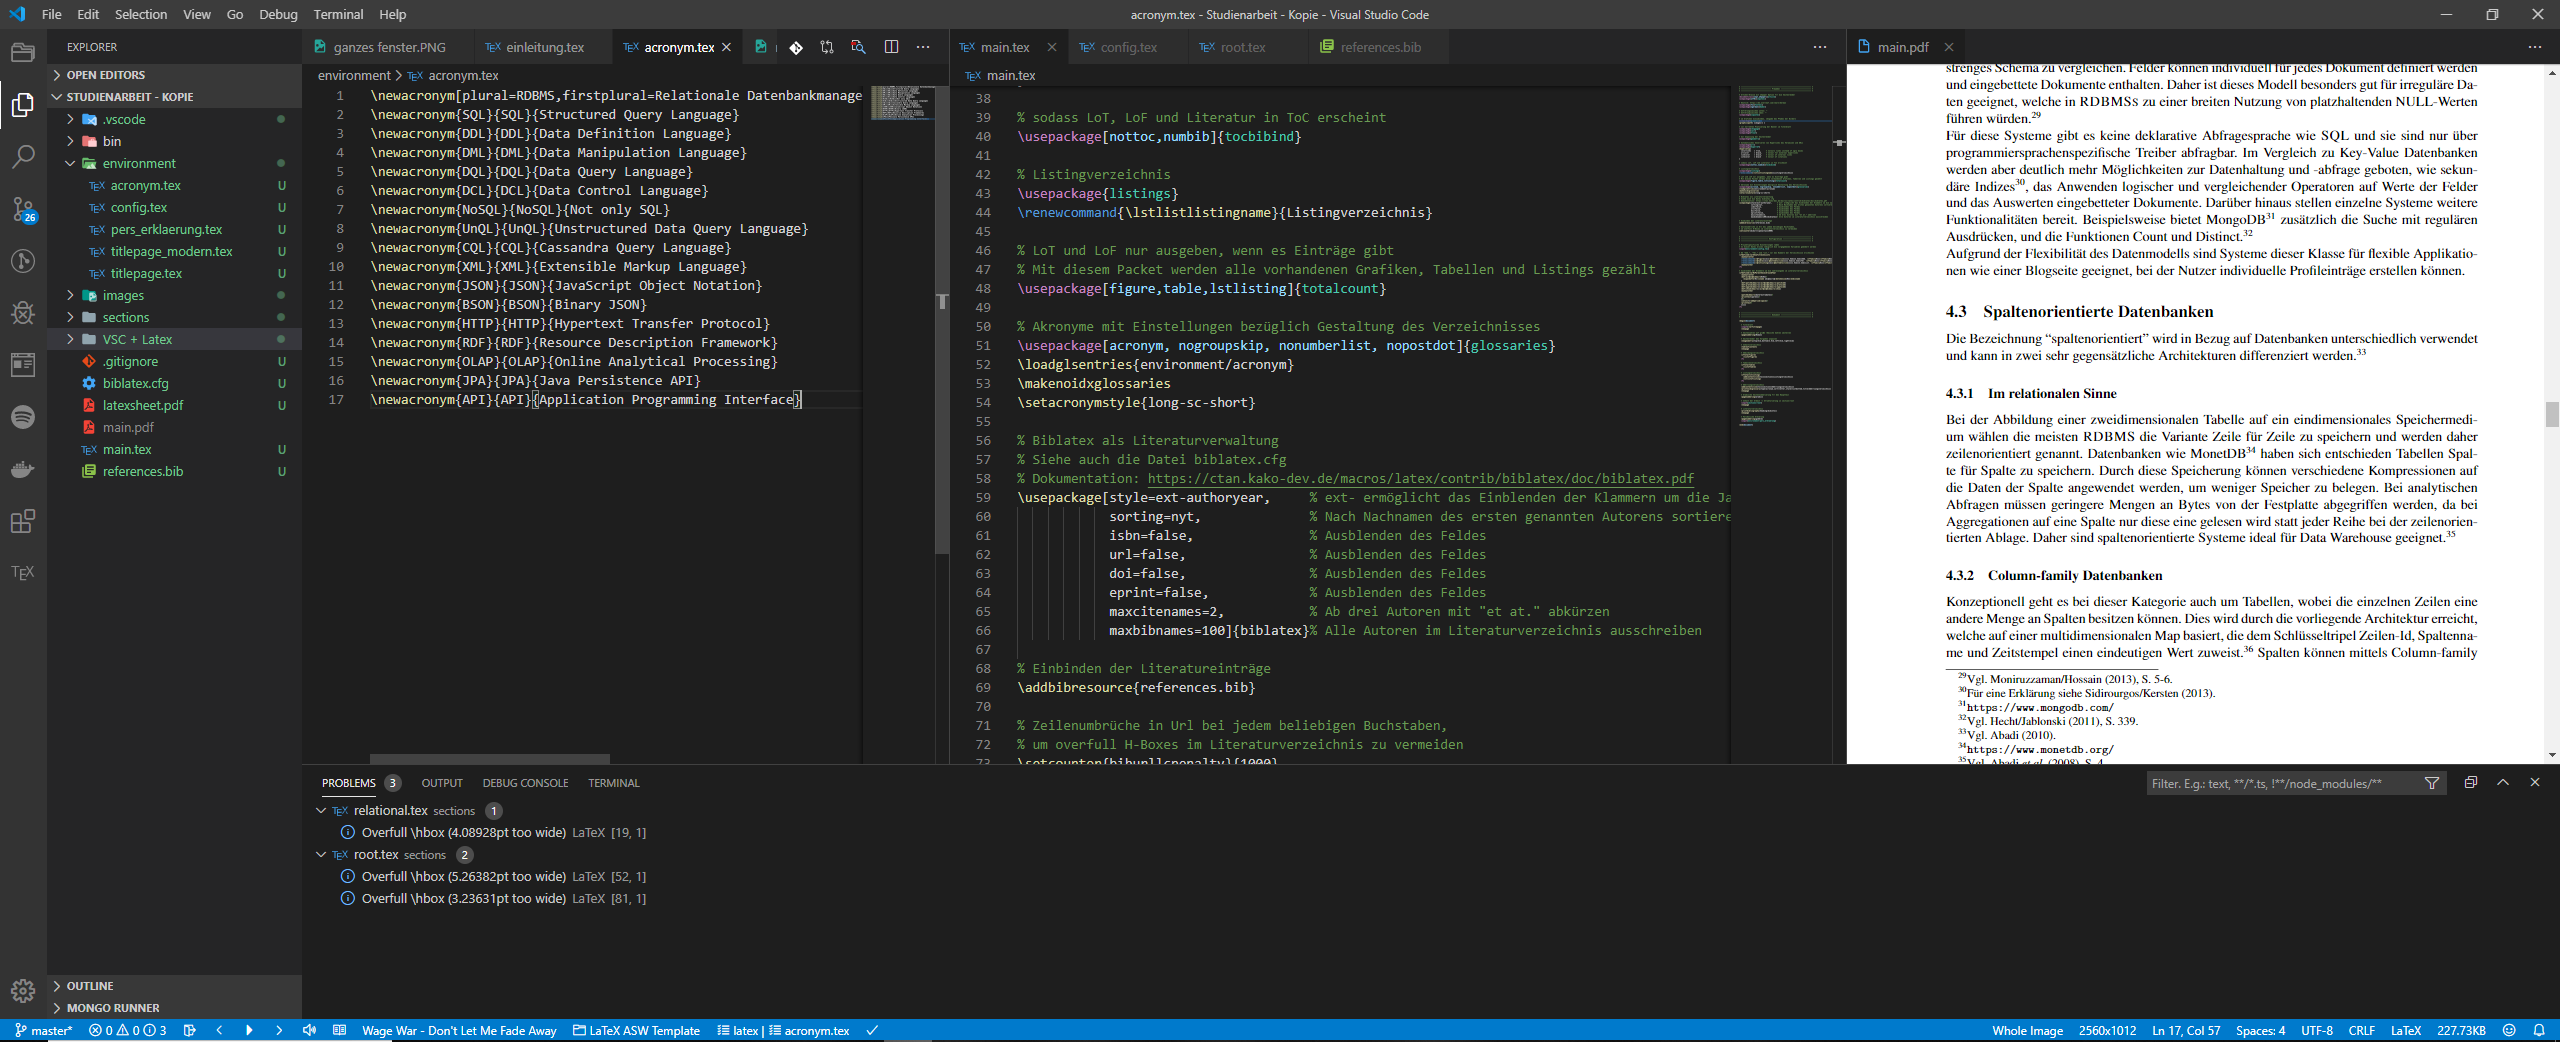
\includegraphics[width=\textwidth]{vsc_latex_workshop}
      \caption{Einblick in die Entwicklungsumgebung Visual Studio Code}
      \label{fig_prototyp_desktop}
    \end{figure}

\subsubsection{Tabellen}
  Tabellen funktionieren wie die erste Art von Bildern; als fließendes Blockelement.

  \begin{table}[bh]
    \centering
    \begin{tabular}{@{}lcccccc@{}}
    \toprule
    Abteilung               & Marketing & Vertrieb & Produktion & IT \\ \midrule
    Besetzte Stellen        & 11        & 16       & 31         & 4  \\
    Unbesetzte Stellen      & 1         & 2        & 0          & 2  \\
    Neu geschaffene Stellen & 3         & 1        & 0          & 2  \\
    Geplante neue Stellen   & 2         & 0        & 2          & 0  \\ \bottomrule
    \end{tabular}
    \caption{Übersicht besetzter und geplanter Stellen im Unternehmen}
    \label{tbl_proglang}
  \end{table}

\subsection{Zitate}
  In \LaTeX gibt es verschiedene Arten wörtlich zu zitieren.
  Zum einen kann es inline durch einfache Anführungszeichen gemacht werden, 
  zum anderen gibt es eine fertige Umgebung, welche das Zitat im Dokument besonders hervorhebt.
  
  \subsubsection{Inline Zitat}
    "`\gls{AWATAD}"'\footcite[S. 2703]{timmerer2019journey}, zu deutsch überall, jederzeit, auf jedem Gerät,
    sind die heutigen Erwartungen der Nutzer im Kontext von Webapplikationen.
    \vgl{timmerer2019journey}{S. 2703--2704}    
    Hierbei ist auf die Codierung der Anführungszeichen zu achten.
  
  \subsubsection{Blockzitat}
    Balzert definiert Softwaretechnik als
    \begin{quotation}
      "`Zielorientierte Bereitstellung und systematische Verwendung von Prinzipien, Methoden und Werkzeugen 
      für die arbeitsteilige, ingenieurmäßige Entwicklung und Anwendung von umfangreichen Softwaresystemen."'\footcite[S. 17]{balzert2010lehrbuch}    
    \end{quotation}
    Dabei betont er, dass etablierte Prinzipien und Methoden, sogenannte 
    \emph{Best Practices}\footnote{\emph{engl.} empfohlene Vorgehensweise},
    an Stelle von eigen erfundenen Muster zu verwenden sind.
    Des Weiteren grenzt er Technologien wie Betriebssysteme, Netzwerke und Datenbanken als Randbereiche ab. 
    Softwareentwicklung ist also die Gesamtheit aller Schritte von der Anforderungsanalyse bis hin zur Wartung eines Softwaresystems
    und lässt sich in die Teildisziplinen \emph{Softwareentwicklung}, \emph{Softwaremanagement} und \emph{Softwarequalitätsmanagement} untergliedern.
    \wholesection{balzert2010lehrbuch}{S. 17--19}

\subsection{Textstrukturierung}
  \subsubsection{Gliederungsebenen}
    In der verwendeten Article-Dokumentenklasse werden standardmäßig 3 Hierarchieebenen unterstützt.
    Diese werden in folgender Aufzählung-Umgebung kurz erläutert.
    
    \begin{itemize}
      \item sections stellen die oberste Ebene dar und werden in dieser Demo in der root.tex Datei definiert.
      \item subsection sind eins drunter
      \item darunter folgt subsubsection, wofür dieses Kapitel ein Beispiel ist 
    \end{itemize}

    \paragraphheader{Bonusebene}
    Falls - wie hier - mehr Gliederungsebenen benötigt werden, als die Dokumentklasse zulässt, 
    kann mittels dem vordefinierten paragraphheader-Befehl eine weitere, unnummerierte Ebene eingefügt werden.
   
  \subsubsection{Mathe-Modus}
    Der Mathe-Modus, der bekanntlich für Formeln genutzt wird lässt sich durch \$ einfach anstellen.

    $http{:}//[\langle benutzer\rangle[{:}\langle passwort\rangle]@]host[{:}\langle port\rangle][/\langle pfad\rangle][?\langle parameter\rangle][\#\langle fragment\rangle]$
    \footcite[Für den Standard URL siehe][]{WHATWGURL}